%!TEX root = ../main.tex
%% Chapter 2 - Openstack


\chapter{OpenStack}

This section gives a detailed description of the \textit{OpenStack} technology in order to better understand how it works.


%%--------------- section
\section{Definition}
\textit{OpenStack} is an open source project licensed under the \textit{Apache License 2.0} and consists of several projects (or services), which allow creating cloud infrastructures.
In other words it is \textit{a cloud operating system that controls large pools of compute, storage, and networking resources throughout a data center, all managed through a dashboard that gives administrators control while empowering their users to provision resources through a web interface.
}\cite{osdef}
Thus, OpenStack provides an out of the box IaaS solution.

%Different projects (or services) offered by OpenStack can be installed separately on different machines, but they are working together.
\rp{try to avoid passive form in your text where possible, it sounds bad, compare with your sentence in the comment above.}
OpenStack offers different services that can be distributed across different machines in various configurations.
A list of these projects is given in the Table \ref{table:openstack_services_list}.
Only the projects Nova, Keystone, Horizon, Glance and Cinder were used for the experiments and will be discussed in more details below.
Figure \ref{fig:openstack_services_arch} shows how each service interacts with other services in a typical OpenStack environment.

%%--------------- section
\section{Services}

In this section, the different services used for the experiments are discussed in details.

\begin{figure}[h]
	\centering
	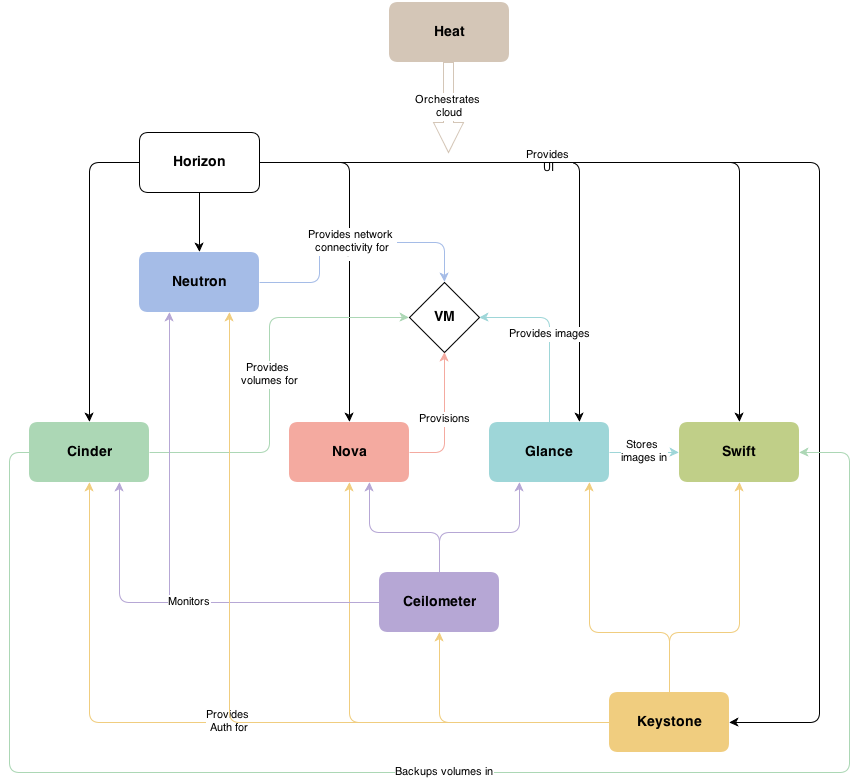
\includegraphics[scale=0.5]{figures/openstack_havana_conceptual_arch.png}
	\caption{Conceptual architecture of OpenStack Havana \cite{osarch}}
	\label{fig:openstack_services_arch}
\end{figure}

\begin{table}[h]
	\centering
	\begin{tabular}{|l|l|p{9.5cm}|}
		\hline
		\textbf{Project name} & \textbf{Service} & \textbf{Description}\\
		\hline
		Nova & Compute & Creates and manages virtual machines\\
		Keystone & Identity & Provides authentication and authorization\\
		Horizon & Dashboard & Web interface to manage all services\\
		Neutron & Networking & Manages networking for advanced network topologies\\
		Glance & Image & Provides a registry of virtual machine images\\
		Cinder & Block Storage & Provides persistent storage to VMs\\
		Swift & Object Storage & Stores data, including virtual images\\
		Ceilometer & Telemetry & Collects metering data (CPU and network costs)\\
		Heat & Orchestration & Generates running cloud applications \rp{I don't understand this}\\
		Trove & Database & Provides scalable and reliable cloud provisioning functionality for relational and non-relational database engines\\
		\hline
	\end{tabular}
	\caption{OpenStack services}
	\label{table:openstack_services_list}
\end{table}

\subsection{Nova}
Nova service is responsible for creating and managing virtual machines on demand.
Upon creating a virtual machine, the user can specify a flavor he wants to use.
The flavor allows to set the characteristics of a virtual machine: amount of RAM, number of virtual CPUs (VCPUs), sizes of root disk, ephemeral disk and swap disk. By default, Nova provides a set of flavors and the user can create more if needed.
Table \ref{table:flavors_list} shows characteristics for a list of the default flavors (ephemeral and swap disks are set to 0).

\begin{table}[h]
	\centering
	\begin{tabular}{|l|l|l|l|}
		\hline
		\textbf{Flavor} & \textbf{# of VCPUs} & \textbf{Disk size (GB)} & \textbf{RAM size (MB)}\\
		\hline
		m1.tiny & 1 & 1 & 512 \\
		m1.small & 1 & 20 & 2048 \\
		m1.medium & 2 & 40 & 4096 \\
		m1.large & 4 & 80 & 8192 \\
		m1.xlarge & 8 & 160 & 16384 \\
		\hline
	\end{tabular}
	\caption{Flavors}
	\label{table:flavors_list}
\end{table}

OpenStack provides two different services to manage storage, namely \textit{Block Storage} and \textit{Object Storage}.
As mentioned earlier, the different OpenStack services can be installed separately, and one does not need to install all the services in order to have a virtual machine running.
\rp{you use phrases like ``said later''/``earlier'' way too often, try to reduce, I've already cut some.}
By default, when creating a virtual machine, it will have its own storage (i.e. a disk or a root disk), which is mandatory in order to install an operating system on it,
and it does not need the Block Storage service. 
The latter will be useful when one needs to extend the storage of a virtual machine in the future. 
Coming back to flavors, ephemeral disk corresponds to the amount of disk space to use for the ephemeral partition when a virtual machine is launched. 
These type of disks are bonded to the lifecycle of a virtual machine, meaning that if a virtual machine is terminated, all the data on the disk are lost. 
However, the data persist after rebooting a virtual machine. 
The root disk is nothing but a special case of ephemeral disk. 
It is used for the root partition (/) and unlike ephemeral disk, it is included in snapshots of virtual machine. 
If the size of the root disk is set to 0, this means that its size will be set to the one of image containing the operating system.
Finally, there is also the possibility to add a swap disk to the virtual machine.
The different storage solutions of OpenStack are summarized in Table \ref{table:storage_list}.

Nova is also able to handle networking thanks to the \texttt{nova-network} service. 
In this case, we talk about \textit{Legacy Networking} rather than \textit{OpenStack Networking} which refers to the Neutron project of OpenStack. 
As networking is very complex, it has been decided to split the Nova project in two parts: one project, Nova, will be exclusively responsible for virtual machines and another project, Neutron, will be exclusively responsible for networking. 
For our experiment, it was sufficient to only use Nova to manage networking instead of Neutron.


\begin{table}[h]
	\centering
	\begin{tabular}{|m{2cm}|m{3.8cm}|m{3.8cm}|m{3.8cm}|}
		\hline
		 & 
		\textbf{Ephemeral \newline storage} & 
		\textbf{Block storage} & 
		\textbf{Object storage}\\
		\hline
		\textbf{Used to} & 
		Run operating system and scratch space & 
		Add additional persistent storage to a virtual machine (VM) & 
		Store data, including VM images \\
		\hline
		\textbf{Accessed through} & 
		A file system & 
		A block device that can be partitioned, formatted, and mounted (such as, /dev/vdc) & 
		The REST API \\
		\hline
		\textbf{Accessible from} & 
		Within a VM & 
		Within a VM & 
		Anywhere \\
		\hline
		\textbf{Managed by} & 
		OpenStack Compute (nova) & 
		OpenStack Block Storage (cinder) & 
		OpenStack Object Storage (swift) \\
		\hline
		\textbf{Persists until} & 
		VM is terminated & 
		Deleted by user & 
		Deleted by user \\
		\hline
		\textbf{Sizing determined by} & 
		Administrator configuration of size settings, known as flavors & 
		User specification in initial request & 
		Amount of available physical storage \\
		\hline
		\textbf{Example of typical usage} & 
		10 GB first disk, 30 GB second disk & 
		1 TB disk & 
		10s of TBs of dataset storage \\
		\hline
	\end{tabular}
	\caption{Storage \cite{stodec}}
	\label{table:storage_list}
\end{table}


\subsection{Glance}
Glance is responsible for providing a registry of virtual machine images. 
The user is then able to easily retrieve an actual image for his virtual machine. 
An image contains an operating system image, which will be used to launch a virtual machine. 
The uploaded images are stored on the same system that hosts the Image Service, in the directory \texttt{/var/lib/glance/images/} by default.

\subsection{Cinder}
Cinder is responsible for providing persistent storage to virtual machines. 
The persistent storage is also called volume. 
Unlike ephemeral storage that was discussed before, all data that are on a volume persist when a virtual machine is terminated. 
This volume is similar to the Amazon Elastic Block Storage (EBS) 
and can be compared to an external hard disk drive (HDD) that is plugged into a computer: we say that the volume is attached to an instance. 
In order for the attached volume to be usable, it has to be mounted and formatted. 
After these steps, files can be stored on the volume. 
The attached volume can also be bootable, and thus replace the root disk seen before.
It has to be noted that one volume can only be attached to one instance at a time, but one instance can have several volumes attached to it.


\subsection{Keystone}
Keystone is responsible for providing authentication and authorization for the other OpenStack services and users. 
Therefore, it offers \textit{User management} and \textit{Service management}. 

The \textit{User management} lets one create users and tenants (or projects), the latter representing a group of users. 
The users will be able to connect to OpenStack by giving their credentials.
It is easy to have an overview of all running instances for the current tenant.
Also, it is possible to give specific roles to the users in a given tenant, so it's easy to restrict a user to only create instances for example. 

In order to manage services, the administrator has to first create a user per service. 
The \textit{Service management} provides identity, token, catalog and policy services.


% \begin{figure}[h]
% 	\centering
% 	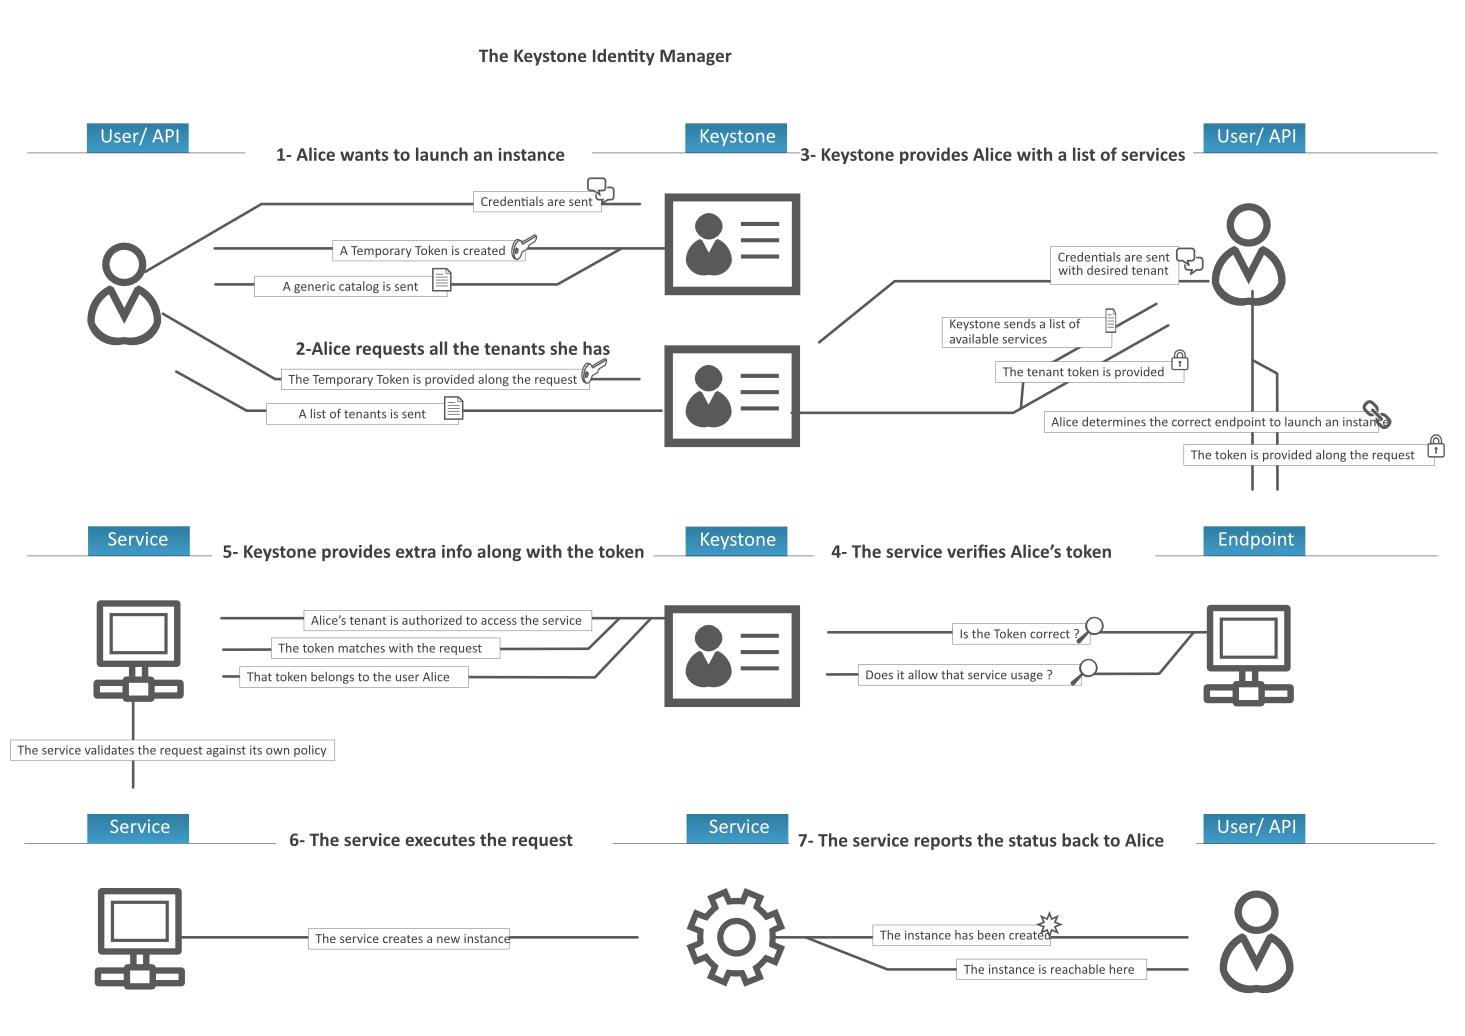
\includegraphics[scale=0.65, angle=90]{figures/keystone.png}
% 	\caption{Identity Service process flow}
% 	\label{fig:openstack_keystone}
% \end{figure} %%% [ref] http://docs.openstack.org/icehouse/install-guide/install/apt/content/keystone-concepts.html

\paragraph{Horizon}\mbox{}\\
Horizon provides a nice web interface (an example is shown in Figure \ref{fig:dashboard}) that lets users and administrators interact with OpenStack services easily, instead of executing commands through a terminal. 
However, Horizon cannot totally replace the command line tool.
Once logged in, users can launch instances and use it directly from a web browser thanks to VNC (or Virtual Network Computing) configured during the installation of OpenStack.








%%--------------- section
\section{Setup}
\label{section_setup}
For our experiments, OpenStack Icehouse was installed and configured on three physical machines:

{
\singlespacing
\begin{itemize}
	\item{\texttt{controller} which acts as a controller node}
	\item{\texttt{compute1} which acts as a compute node}
	\item{\texttt{compute2} which acts as a compute node and a block storage node}
\end{itemize}
}

As installing OpenStack is a relatively long process, all the steps won't be describe in this section. The OpenStack documentation \cite{osinstall}
descibes a well step-by-step that was followed in order to make everything work correctly.


\paragraph{Naming convention}\mbox{}\\
Virtual machines created on \texttt{compute1} will be called \texttt{vm1}, and those created on \texttt{compute2} will be called \texttt{vm2}. Moreover if the virtual machine has a block storage attached to it, \texttt{bs} will be attached to its name, becoming \texttt{vm1bs} for example. This convention will be followed for the rest of this report.


%%--------------- subsubsection
\subsection{Machines}
In this section, the hardware used for the experiments will be presented. We have three physical machines on which OpenStack services are installed, and several virtual machines with different flavors will be created on the physical machines with OpenStack.


\paragraph{Physical machines}\mbox{}\\
The three physical machines briefly presented in Section \ref{section_setup} are HP Compaq Elite 8300 SFF with a 64-bit architecture. 
Each machine uses a 3.4 GHz Intel Core i7-3770. 
There is 16GB of RAM, $4\times4$GB DIMM DDR3 Synchronous 1600MHz. 
They have a Western Digital HDD of 500GB. 
In the case of \texttt{compute2}, a partition of 100GB (93GB after partioning with GParted) has been created in order to have space for the Block Storage service of OpenStack instead of a full disk recommended by the OpenStack documentation. 
Physical and logical volumes have been created with LVM (Logical Volume Manager) for the partition created.
The machines are running Ubuntu 14.04 LTS 64 bit operating system. 
To create and run virtual machines, the open source hypervisor KVM (Kernel-based Virtual Machine) is used by the Compute Service. Concerning the network, each machine only have one interface card, instead of two interface cards recommended by the OpenStack documentation.



\paragraph{Virtual machines}\mbox{}\\
The virtual machines are created on \texttt{compute1} and \texttt{compute2} only and are using a cloud image\footnote{Ubuntu cloud images can be found here: \url{https://cloud-images.ubuntu.com}} of Ubuntu Server 14.04 LTS made to run on cloud platforms like OpenStack. 
A new flavor called \textit{physical} has been created and the flavor \textit{large} has been modified accordingly. 
The updated list of flavors is now represented on Table \ref{table:flavors_list_2}. 
For the experiments, only \textit{large} and \textit{physical} flavors are relevant. 
With the \textit{physical} flavor, we try to have similar characteristics as a physical machine in order to compare them. 
In this context, only one virtual machine with \textit{physical} flavor will be running at a time. 
With the \textit{large} flavor, we try to have half of characteristics of a physical machine in order to have enough resources to run two virtual machines at the same time to test isolation later.

\begin{table}[h]
	\centering
	\begin{tabular}{|l|l|l|l|}
		\hline
		\textbf{Flavor} & \textbf{VCPUs} & \textbf{Disk (in GB)} & \textbf{RAM (in MB)}\\
		\hline
		m1.tiny & 1 & 1 & 512 \\
		m1.small & 1 & 20 & 2048 \\
		m1.medium & 2 & 40 & 4096 \\
		m1.large & 4 & 30 & 8192 \\
		physical & 7 & 30 & 13312 \\
		\hline
	\end{tabular}
	\caption{Flavors}
	\label{table:flavors_list_2}
\end{table}



%%--------------- subsubsection
\subsection{OpenStack services} % TODO: or Components installation (?)
In this section, we will briefly explained which OpenStack services are installed on which physical machines and their purposes. The repartition of the different compoenents is shown in Figure \ref{fig:os_arch}.

\begin{figure}[h]
	\centering
	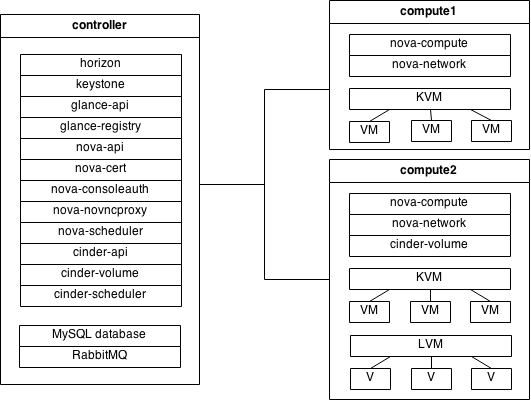
\includegraphics[scale=0.6]{figures/os_arch.png}
	\caption{Our OpenStack architecture}
	\label{fig:os_arch}
\end{figure}

First, let's take a look at \texttt{controller}. 
As its name suggests it, the controller node is the heart of our OpenStack architecture, and thus all the different services APIs (Application Programming Interface) are installed on it. 
Indeed, Keystone is there to manage users, and thus OpenStack services, as a user is created for each service. 
Each request made by a service is handled by Keystone first: the service must authenticate against Keystone, if this succeeds, then permissions are also checked, and if this is okay, the request is accepted and further actions can be done by the service who correctly authenticated itself. 
Glance (\textit{glance-api} and \textit{glance-registry}) is also installed on the controller node. 
This means that all actions regarding images (creation, edition, deletion) are handled by the controller node. 
Moreover all the different images are stored on it.
% TODO: put this text and the image in chapter 1 ?
A web interface makes OpenStack easier to use, and for that Horizon will be installed on the controller node, letting one access OpenStack with the following link \url{http://diufpc117.unifr.ch/horizon}\footnote{Access restricted to unifr network}. 
An overview of the dashboard is shown in Figure \ref{fig:dashboard}. 
As it can be seen, the dashboard offers access to each service installed, and as an administrator, it is possible to manage anything. 
To create, edit and delete an instance, a volume or an image, the user will access to these services through the \textit{Project} tab.
%
\begin{figure}[h]
	\centering
	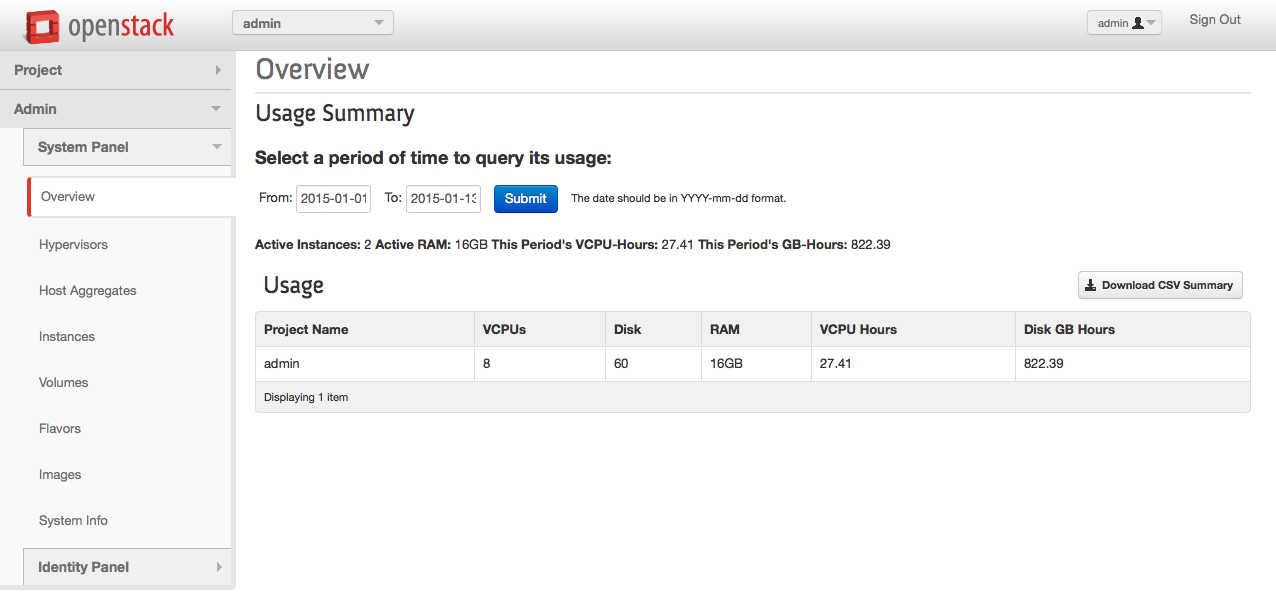
\includegraphics[scale=0.36]{figures/dashboard.png}
	\caption{Dashboard overview}
	\label{fig:dashboard}
\end{figure}
%
%TODO: nova -> describe each service?
In order to be able to create virtual machines, some components of Nova have to be installed on the controller node. These components are there for managing purpose. 
Among them, we can mention \textit{nova-api}, \textit{nova-cert}, \textit{nova-consoleauth} and \textit{nova-novncproxy} for accessing an instance via VNC, and \textit{nova-scheduler} to determine on which physical machine an instance will run.
Likewise, \textit{cinder-api}, \textit{cinder-volume} and \textit{cinder-scheduler} components of Cinder are installed on the controller for management purpose.
As each OpenStack needs to store some information, a database is necessary. 
For this a MySQL database is installed and configured on the controller node. 
On any additional node (in our case, on \texttt{compute1} and \texttt{compute2}), only a MySQL client is installed to access the database hosted on the controller node.
%TODO: messaging system?


Compared to the controller node, \texttt{compute1} and \texttt{compute2} are less complex and don't need to run as many services as the controller. 
For \texttt{compute1}, as its role is to create and host the virtual machines, other compoenents of the Nova project are needed: \textit{nova-compute}, which is responsible for creating and terminating virtual machines, and \textit{nova-network}, which is responsible for managing the network (bridging, updating iptables rules) for the virtual machines. 

Finally, \texttt{compute2} has the same compoenents as \texttt{compute1} regarding the Nova project. 
As this node also needs to take care of the creation and deletion of volumes, the \textit{cinder-volume} component of the Cinder project is present on the node. 


